% Global vs local maximum on a utility surface — MATLAB-style surf plot
% build: pdflatex fig-optimum-surface.tex
\documentclass[border=2pt]{standalone}
\usepackage[T1]{fontenc}
\usepackage{lmodern}
\usepackage{amsmath}
\usepackage{bm}
\usepackage{tikz}
\usepackage{pgfplots}
\usetikzlibrary{calc}
\pgfplotsset{compat=1.18}
\usepgfplotslibrary{colormaps}

\begin{document}
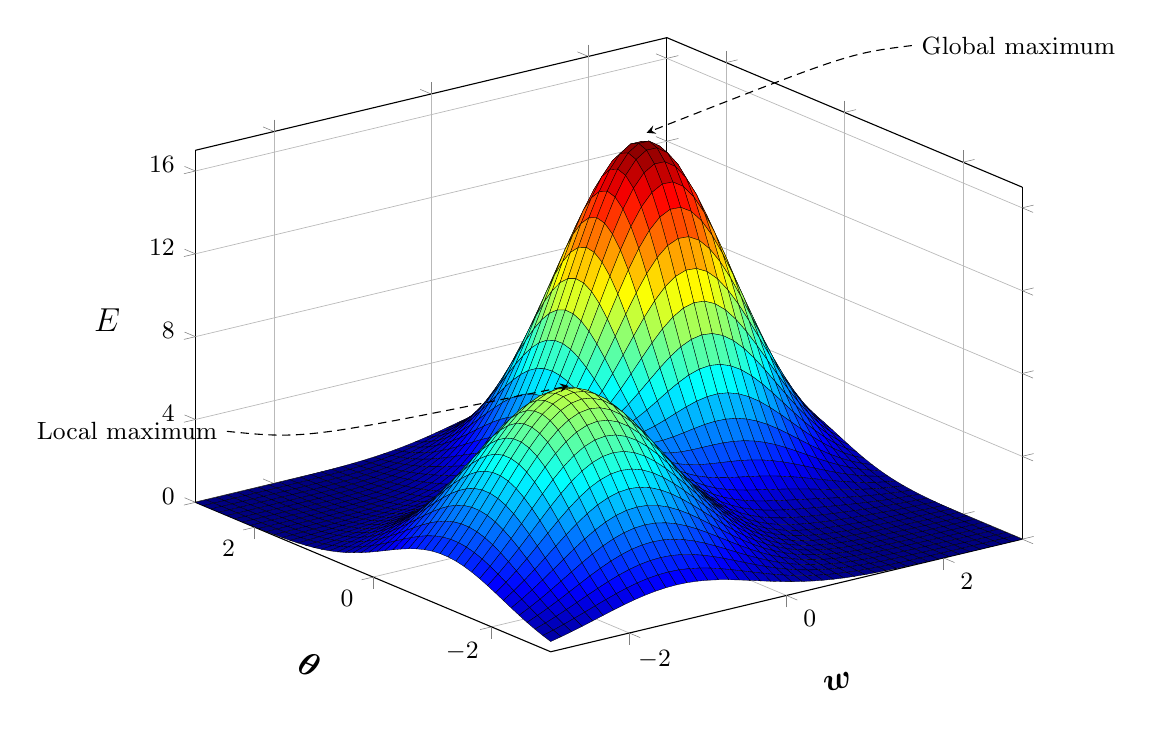
\begin{tikzpicture}
\begin{axis}[
  width=105mm, height=78mm, scale only axis,
  view={-37}{28},
  colormap/jet,
  grid=both,
  grid style={gray!55, line width=0.25pt},
  xmin=-3, xmax=3, ymin=-3, ymax=3, zmin=0, zmax=17,
  xtick={-2,0,2}, ytick={-2,0,2}, ztick={0,4,8,12,16},
  xlabel={$\bm{w}$}, ylabel={$\bm{\theta}$}, zlabel={$E$},
  xlabel style={sloped like x axis, font=\large, yshift=-2mm},
  ylabel style={sloped like y axis, font=\large, yshift=-2mm},
  zlabel style={rotate=-90, font=\large, xshift=-1mm},
  tick label style={font=\small},
  axis line style={line width=0.4pt, black},
  tick align=outside,
  clip=false,
]

% E(w,theta) = 16 * exp(-((w-1.2)^2 + (t-1.0)^2)/1.6)      global maximum
%            +  9 * exp(-((w+1.4)^2 + (t+1.2)^2)/2.0)      local maximum
\addplot3[
  surf, shader=faceted,
  samples=46, domain=-3:3, domain y=-3:3,
  mesh/interior colormap name=jet,
  faceted color=black, line width=0.12pt,
]
{16*exp(-(((x-1.2)^2 + (y-1.0)^2)/1.6))
 + 9*exp(-(((x+1.4)^2 + (y+1.2)^2)/2.0))};

% ---- peak coordinates (labels are placed outside the axis) -----------
\coordinate (gpk) at (axis cs:1.28,1.06,16.30);
\coordinate (lpk) at (axis cs:-1.46,-1.26,9.35);
\end{axis}

\node[anchor=west, font=\small] (glab) at ($(current axis.north east)+(-14mm,-1mm)$)
  {Global maximum};
\draw[densely dashed, line width=0.4pt, -stealth]
  (glab.west) .. controls +(-8mm,-1mm) .. (gpk);

\node[anchor=east, font=\small] (llab) at ($(current axis.west)+(4mm,-11mm)$)
  {Local maximum};
\draw[densely dashed, line width=0.4pt, -stealth]
  (llab.east) .. controls +(10mm,-1mm) .. (lpk);
\end{tikzpicture}
\end{document}
